%<dscrpt>Plan projectif fini.</dscrpt>
On appelle \emph{plan projectif fini} un ensemble fini $\Pi$ (de cardinal $p$) muni d'une partie $\Delta$ de $\mathcal{P}(\Pi)$ vérifiant un certain nombre de propriétés. Les éléments de $\Pi$ sont appelés des \emph{points}, les éléments de $\Delta$ sont appelés des \emph{droites}. Les droites sont des ensembles de points.\newline
Les conditions imposées sont les suivantes.
\begin{itemize}
 \item Si $a$ et $b$ sont deux points distincts de $\Pi$, il existe une unique droite les contenant. Cette droite sera notée $D(a,b)$.
 \item L'intersection de deux droites distinctes est \emph{toujours} un singleton.
 \item Il existe quatre points distincts $a_1$, $a_2$, $a_3$, $a_4$ tels qu'aucune droite ne contienne trois de ces points. 
\end{itemize}
\begin{figure}[h!t]
 \centering
 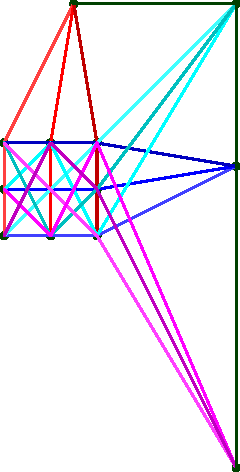
\includegraphics{./Enbppf_1.pdf}
 % Enbppf_1.pdf: 0x0 pixel, 0dpi, 0.00x0.00 cm, bb=
 \caption{Une représentation d'un plan projectif fini}
 \label{fig: Enbppf_1}
\end{figure}

\begin{enumerate}
 \item Combien de parties à deux éléments peut-on former dans un ensemble à $4$ éléments ? En déduire qu'il existe au moins $6$ droites distinctes.
 \item Montrer que $\Pi$ n'est pas l'union de deux droites.
 \item Soit $\delta$ et $\delta'$ deux droites distinctes et $O$ un point n'appartenant à aucune des deux. On définit une application
\begin{displaymath}
 f: 
\left\lbrace 
\begin{aligned}
 \delta &\rightarrow \delta' \\
 a &\mapsto \text{ l'unique point de } D(O,a)\cap \delta'
\end{aligned}
\right. 
\end{displaymath}
Montrer que cette application est bijective. On en déduit que toutes les droites ont le même nombre d'éléments noté $d$.
\item Soit $O$ un point du plan et $n_O$ le nombre de droites passant par $O$. En classant les points de $\Pi\setminus\left\lbrace O \right\rbrace$ suivant la droite passant par $O$ à laquelle ils appartiennent, former une relation entre divers nombres d'éléments. Que peut-on en déduire pour les $n_O$ lorsque $O$ varie dans le plan ?
\item Montrer que le nombre de droites passant par un point est égal au nombre de points sur une droite.
\item Montrer qu'il existe un entier $n$ tel que
\begin{itemize}
 \item Le nombre de points sur une droite est égal au nombre de droites passant par un point et que ce nombre est $n +1$.
 \item Le nombre de points est égal au nombre de droites et que ce nombre est $n^2+n+1$.
\end{itemize}
 
\end{enumerate}

